\documentclass[final]{beamer}  
  \mode<presentation> { \usetheme{ParisSaclay}  }
  \usepackage[english]{babel}
  \usepackage[latin1]{inputenc}
  \usepackage{amsmath,amsthm, amssymb, latexsym}

 
  %\usefonttheme[onlymath]{serif}
  \boldmath %math en gras
  \usepackage[orientation=portrait,size=a0,scale=1.4,debug]{beamerposter}                       % e.g. for DIN-A0 poster
  %\usepackage[orientation=portrait,size=a1,scale=1.4,grid,debug]{beamerposter}                  % e.g. for DIN-A1 poster, with optional grid and debug output
  %\usepackage[size=custom,width=200,height=120,scale=2,debug]{beamerposter}                     % e.g. for custom size poster
  %\usepackage[orientation=portrait,size=a0,scale=1.0,printer=rwth-glossy-uv.df]{beamerposter}   % e.g. for DIN-A0 poster with rwth-glossy-uv printer check
  % ...
  \usepackage{graphicx}
  \usepackage{tikz}
  \usepackage{lipsum} % remove if not used
  
%\setbeamertemplate{background canvas}{\includegraphics[width=\paperwidth]{}}
% you may add a backgroud color or image
 %
  \title{\huge Poster template for Universit\'e Paris-Saclay}
  \author{Name Author 1, Name Author 2}
  \institute[]{Laboratory Name, Faculty/School, adress}

\begin{document}

\begin{frame} [fragile]{} 

 
\begin{columns}
    % ---------------------------------------------------------%

    \begin{column}{.4\textwidth}
        %
    \begin{block}{Recommandations}
    \large This template is compliant with the official charter, you can change anything at your convenience, providing you keep the prune color  \normalsize (\texttt{CMJN 24 100 17 60 -- RVB 99 0 60 -- HEX 63003C}) \large as main color 'especially the background of the title box) and you use only colors from the charter \small  \texttt{ https://www.universite-paris-saclay.fr/luniversite /media-et-communication/logos-de-luniversite-paris-saclay}
    %\lipsum[1][1-2]
    
       \begin{itemize}
       		\item do not change \texttt{beamerposter.sty} unless you know what you are doing,
       		\item you can change  \texttt{beamerthemeParisSaclay.sty}, you can add colors from the charter, but do not change alredy defined colors,
       		\item change other affiliation logos and conference references in \texttt{beamerthemeParisSaclay.sty}
       \end{itemize}
  	%\lipsum[1][11-18]
   \end{block}
\vspace{1cm}
		\begin{alertblock}{Alert block}
			\[\vec \nabla \vec H = \vec j + \frac{d \vec D}{dt}\]
			
			\[ {F}=\mu_0\chi H \frac{dH}{dx} \]
		\end{alertblock}
		
		\bigskip
		
	\begin{block}{Block, normal type}
	\begin{figure}
	\begin{tikzpicture}[scale=.95]
		\draw [domain=0:29,samples=50,ultra thick,rouge] plot [mark=*,mark size=5] (\x,{18-18/((\x/3)^2+1)});
		\draw (0,0)rectangle(30,20) ;
		\foreach \o in {0,2,...,20} \draw(-1,\o)node[left]{\o};
		\foreach \a in {0,1,...,15} \draw(\a*2,0)node[below]{\a};

	\end{tikzpicture}
	\caption{Magnetization vs. field of some ferromagnetic material (a.u.)}
	\end{figure}
	\lipsum[1][1-2]
	\end{block}
	\vspace{1cm}
	\begin{block}{Titre de bloc}
	\begin{figure}
	\begin{tikzpicture}[scale=2]
		\fill [black] (0,-4) rectangle (10,4);
		\draw [very thin, gray] (0,-4) grid (10,4);
		\draw [domain=0:10,samples=200,ultra thick,vertl] plot (\x,{2*sin(\x*60)+sin(\x*720)/2});
		\draw [domain=0:10,samples=100,thick,mandarine] plot (\x,{2*sin(\x*60-30)});
	\end{tikzpicture}
	\caption{Oscilloscope display}
	\end{figure}
	 \lipsum[1][3-4]
	\end{block}
	  
	\end{column}
	
% ---------------------------------------------------------%

    \begin{column}{.4\textwidth}	
	\begin{exampleblock}{Example block}
	\lipsum[3]
	\end{exampleblock}
	
\vspace{1cm}		
	
	\begin{block}{Campus vue}
	\begin{figure}
	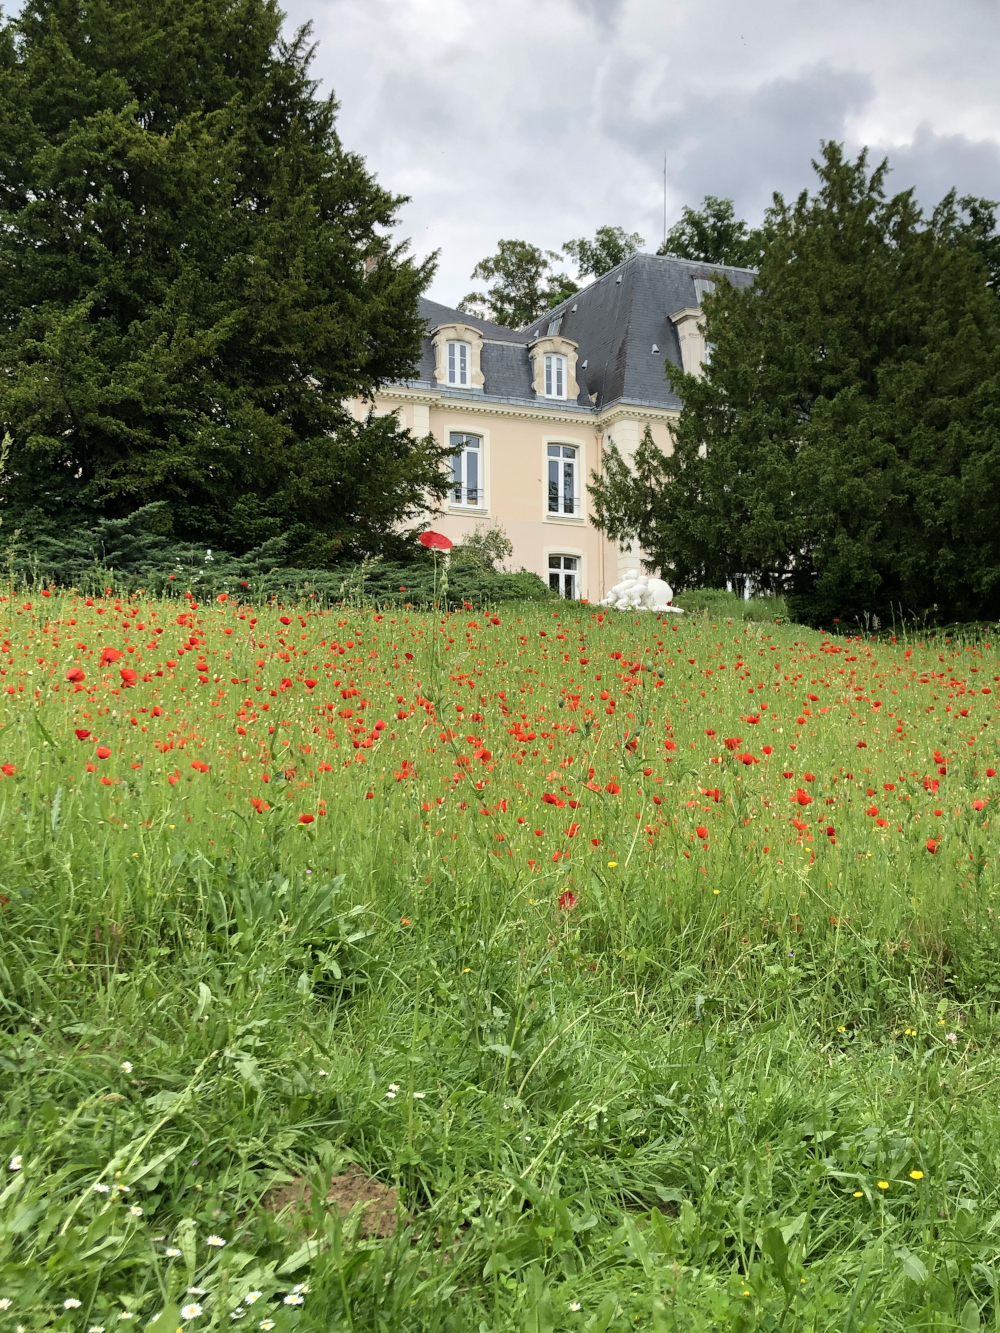
\includegraphics[width=.9\textwidth]{300} 	
	\caption{Vue of building 300, aka "le chateau"}
	
	\end{figure}
	
	\lipsum [4][1-4]
	\end{block}
	
	\vspace{1cm}	

		\begin{exampleblock}{Bibliography}
			\begin{enumerate}
       			\item James Clerk Maxwell, \textit{A treatese on electricity and magnetism}, Clarendon Press, Oxford 1873.
       			\item Pierre Curie, \textit{Propri\'et\'es magn\'etiques des corps \`a diverses temp\'eratures}, PhD. thesis, Sorbonne University, Paris, 1895
       			\item James Alfred Ewing, \textit{Magnetic induction in iron and other metals}, D. Van Nostrand Company, 1901.
       		\end{enumerate}

\vspace{1cm}		
		
		\end{exampleblock}
		
		\begin{exampleblock}{Acknowlegements}
			This projet was founded by some institution under the grant number XX-0000
		
		\end{exampleblock}

	\end{column}
\end{columns}




    
\end{frame}

\end{document}